\documentclass[a4paper,11pt]{article}
\usepackage{amsmath,amsthm,amsfonts,amssymb,amscd,amstext,vmargin,graphics,graphicx,tabularx,multicol} 
\usepackage[francais]{babel}
\usepackage[utf8]{inputenc}  
\usepackage[T1]{fontenc} 
\usepackage{pstricks-add,tikz,tkz-tab,variations}
\usepackage[autolanguage,np]{numprint} 

\setmarginsrb{1.5cm}{0.5cm}{1cm}{0.5cm}{0cm}{0cm}{0cm}{0cm} %Gauche, haut, droite, haut
\newcounter{numexo}
\newcommand{\exo}[1]{\stepcounter{numexo}\noindent{\bf Exercice~\thenumexo} : \marginpar{\hfill /#1}}
\reversemarginpar


\newcounter{enumtabi}
\newcounter{enumtaba}
\newcommand{\q}{\stepcounter{enumtabi} \theenumtabi.  }
\newcommand{\qa}{\stepcounter{enumtaba} (\alph{enumtaba}) }
\newcommand{\initq}{\setcounter{enumtabi}{0}}
\newcommand{\initqa}{\setcounter{enumtaba}{0}}

\newcommand{\be}{\begin{enumerate}}
\newcommand{\ee}{\end{enumerate}}
\newcommand{\bi}{\begin{itemize}}
\newcommand{\ei}{\end{itemize}}
\newcommand{\bp}{\begin{pspicture*}}
\newcommand{\ep}{\end{pspicture*}}
\newcommand{\bt}{\begin{tabular}}
\newcommand{\et}{\end{tabular}}
\renewcommand{\tabularxcolumn}[1]{>{\centering}m{#1}} %(colonne m{} centrée, au lieu de p par défault) 
\newcommand{\tnl}{\tabularnewline}

\newcommand{\bmul}[1]{\begin{multicols}{#1}}
\newcommand{\emul}{\end{multicols}}

\newcommand{\trait}{\noindent \rule{\linewidth}{0.2mm}}
\newcommand{\hs}[1]{\hspace{#1}}
\newcommand{\vs}[1]{\vspace{#1}}

\newcommand{\N}{\mathbb{N}}
\newcommand{\Z}{\mathbb{Z}}
\newcommand{\R}{\mathbb{R}}
\newcommand{\C}{\mathbb{C}}
\newcommand{\Dcal}{\mathcal{D}}
\newcommand{\Ccal}{\mathcal{C}}
\newcommand{\mc}{\mathcal}

\newcommand{\vect}[1]{\overrightarrow{#1}}
\newcommand{\ds}{\displaystyle}
\newcommand{\eq}{\quad \Leftrightarrow \quad}
\newcommand{\vecti}{\vec{\imath}}
\newcommand{\vectj}{\vec{\jmath}}
\newcommand{\Oij}{(O;\vec{\imath}, \vec{\jmath})}
\newcommand{\OIJ}{(O;I,J)}


\newcommand{\reponse}[1][1]{%
\multido{}{#1}{\makebox[\linewidth]{\rule[0pt]{0pt}{20pt}\dotfill}
}}

\newcommand{\titre}[5] 
% #1: titre #2: haut gauche #3: bas gauche #4: haut droite #5: bas droite
{
\noindent #2 \hfill #4 \\
#3 \hfill #5

\vspace{-1.6cm}

\begin{center}\rule{6cm}{0.5mm}\end{center}
\vspace{0.2cm}
\begin{center}{\large{\textbf{#1}}}\end{center}
\begin{center}\rule{6cm}{0.5mm}\end{center}
}



\begin{document}
\pagestyle{empty}
\titre{Interrogation: Les nombres décimaux}{Nom :}{Prénom :}{6èmeA}{Date}

\begin{flushleft}
\begin{tabular}{|m{9.5cm}|m{1.25cm}|m{1.25cm}|m{1.25cm}|m{1.25cm}|m{1.25cm}|}
\hline 
\textbf{Compétences} & \begin{center}
\textbf{N.E.}
\end{center} & \begin{center}
\textbf{M.I.}
\end{center} & \begin{center}
\textbf{M.F.}
\end{center}  & \begin{center}
\textbf{M.S.}
\end{center} & \begin{center}
\textbf{T.B.M.}
\end{center} \\ 
\hline 
Je dois savoir maîtriser les différentes écritures des nombres décimaux (en lettres, en chiffre et en 
décomposition) &  &  & & &\\
\hline 
Je dois connaître l'écriture décimale d'un nombre et utiliser la valeur de ces chiffres en fonction de leur rang dans l'écriture &  &  & & &\\
\hline
Je dois connaître et utiliser les fractions décimales pour écrire ou décomposer un nombre décimal  &  &  & & &\\ 
\hline

\end{tabular} 
\end{flushleft}

\textit{N.E = Non évalué ; M.I. = Maîtrise insuffisante ; M.F. = Maîtrise fragile ; M.S. = Maîtrise satisfaisante ; T.B.M. = Très bonne maîtrise}\\


\vspace*{0.5cm}

\exo{1} Le nombre 11,564 est-il un nombre décimal ? Expliquer votre réponse en vous aidant de la définition de votre cours.\\
\reponse[4]\\



\exo{1.5}  Réécrire les nombres suivants en supprimant les zéros inutiles (lorsqu'il y en a).\\

\qa  01 205 500,0001 \hspace*{2.5cm}\qa 75,00 \hspace*{2.5cm}\qa 020,020 \\

\hspace*{0.5cm} . . . . . . . . . . . \hspace*{2.7cm} . . . . . . . \hspace*{2.7cm} . . . . . . . \\

\qa 005 410,070 0 \hspace*{2.5cm}\qa 057,040 \hspace*{2.5cm}\qa 003,8 \\

\hspace*{0.5cm}. . . . . . . . . . . \hspace*{3cm} . . . . . . . \hspace*{2.5cm} . . . . . . . \\



\exo{2} On considère le nombre 4 091,807.\\

\initqa \qa Quel est le chiffre des dixièmes ?  . . . . . . . . . . . . . . . . . . . . . . . . . . . . . . . . . . . . . . . . . . . . . . . . . . . . . . \\

\qa Quel est le nombre de centaines ?  . . . . . . . . . . . . . . . . . . . . . . . . . . . . . . . . . . . . . . . . . . . . . . . . . . . \\

\qa Que représente le chiffre 7 ? . . . . . . . . . . . . . . . . . . . . . . . . . . . . . . . . . . . . . . . . . . . . . . . . . . . . . . \\

\qa Que représente le nombre 409 180 ? . . . . . . . . . . . . . . . . . . . . . . . . . . . . . . . . . . . . . . . . . . . . . . . . . . .  \\


\vspace*{0.25cm}
\exo{3} \\

\initq \initqa \q Écrire les nombres suivants avec \textbf{une} fraction décimale.

\bmul {2}

 0,24 = . . . . . \\

\columnbreak


78,102 = . . . . . \\

\emul

\newpage


\q Donner l'écriture décimale des nombres suivants.

\bmul{3}

$ 34 + \dfrac{2}{10} + \dfrac{7}{1000}$ = . . . . . . . . . . . .\\

\columnbreak

$ 6 +  \dfrac{5}{100}$ = . . . . . . . . . . . .\\

\columnbreak

$  \dfrac{7}{10} + \dfrac{8}{1000}$ = . . . . . . . . . . . .\\

\emul

$ (5 \times 100) + (7 \times 1) + (2 \times 0,1) + (3 \times 0,01)+ (9 \times 0,001)$ = . . . . . . . . . . . .\\

\vspace*{0.3cm}

\exo{1.5} Compléter avec des chiffres pour que les égalités soient vraies.\\

\initqa \qa $\dfrac{23}{100} + \dfrac{...}{1000}= \dfrac{\text{... ... } 7}{1000}$\\

\qa 5 ...  + $\dfrac{\text{3 ...}}{100} = \dfrac{\text{... 83 ...}}{\text{... ... ...}} = \text{... ...} +\dfrac{...}{10} +\dfrac{1}{100}$\\

\qa $\dfrac{1 ...}{10} + \dfrac{\text{... 4}}{1000}= \dfrac{\text{... 41 ...}}{1000}$\\

\exo{1}\\

Je suis un nombre décimal avec deux chiffres après la virgule.\\
Mon chiffre des centièmes est le même que celui des millièmes de 925,647.\\
Mon chiffre des dixièmes est le même que celui des centièmes de 6,0371.\\
Ma partie entière est égale à la partie décimale de 853,724. Qui suis-je ?\\

\noindent \reponse[1]\\


\exo{+1} BONUS\\

Compléter la grille ci-dessous.

\begin{center}
\includegraphics[scale=1]{motcroise.eps} 
\end{center}

\textbf{Horizontalement}\\

\noindent \textbf{A.}      $109 \times 100 + 4 \times 10 + 9$\\
\textbf{B.}        La partie entière de 5,02. /  Nombre entier compris entre 
519,9 et  520,2.\\
\textbf{C.}      Le nombre de centièmes dans 0,3. / Combien de nombres entiers y-t-il entre 1257,2 et 1265,9?\\
\textbf{D.}       Le nombre de millièmes dans $25 + \dfrac{7}{100} + \dfrac{4}{10} + \dfrac{1}{1000}$.\\
\textbf{E.}      Trois dizaines. /   6,6 dizaines.\\

\textbf{Verticalement}\\

\noindent \textbf{1.}      Le nombre de dixièmes dans $\dfrac{150}{100}$. / La partie entière de 23,264.\\
\textbf{2.}      Le chiffre des centièmes de 25,007. / Nombre entier compris 
entre 349,05 et 350 ,2.\\
\textbf{3.}      Le nombre de millièmes dans 9,504.\\
\textbf{4.}      420 dixièmes. /  0,76 centaines.\\
\textbf{5.}      $\dfrac{9081600}{100}$.\\



\end{document}
